\documentclass[11pt,twocolumn]{article}
\usepackage[margin=1in]{geometry}
\usepackage{graphicx}
\usepackage{amsmath,amssymb}
\usepackage{hyperref}
\usepackage{natbib}

\title{
\textbf{WISE - Waste Image Sorting and Evaluation}\\
Ensemble CNN Pipeline for Trash Detection and Classification
}
\author{
Brett Castro \\
University of Virginia \\
\texttt{gry6ks@virginia.edu}
\and
Tyler Gorecki \\
University of Virginia \\
\texttt{ttg6nx@virginia.edu}
\and
Vishwanath Guruvayur \\
University of Virginia \\
\texttt{vish@virginia.edu}
\and
Akaash Kamdar \\
University of Virginia \\
\texttt{ak2znr@virginia.edu}
\and
Isaac Levy \\
University of Virginia \\
\texttt{gbz6qn@virginia.edu}
}
\date{}
\begin{document}


\twocolumn[{
\maketitle
%%%%%%%%%% ABSTRACT %%%%%%%%%%%%%%%%%%
\begin{abstract}
Effective waste management is a critical global challenge with far-reaching environmental, economic, and public health implications. Despite increasing awareness, less than 20\% of global waste is currently recycled, resulting in significant resource depletion, environmental degradation, and public exposure to hazardous materials. 

The \textbf{WISE} (Waste Identification and Sorting using Enhanced vision) project addresses this gap by employing deep learning for automated waste classification through image recognition. By enabling accurate and efficient real-time sorting, our system aims to optimize recycling processes, reduce human health risks, and facilitate the recovery of valuable materials. We conducted a comparative analysis of three state-of-the-art convolutional neural networks: ResNet, GoogLeNet, and EfficientNet—on a dataset of 19,762 labeled waste images spanning 10 distinct classes. 


Our evaluation highlights each model’s strengths and limitations in terms of accuracy, efficiency, and robustness, offering actionable insights for deploying AI-driven solutions in real-world recycling infrastructures. This work demonstrates the transformative potential of AI in advancing sustainable waste management practices.
\vspace{1cm}
\end{abstract}

}]



%%%%%%%%%% INTRODUCTION %%%%%%%%%%%%%%
\section{Introduction}

\label{sec:intro}


Improper waste disposal leads to contaminated recycling streams, increased costs, and harm to ecosystems. Currently, annual waste generation exceeds 2 billion tons and is expected to increase by 70\% to 3.4 billion tons by 2050. With this predicted drastic increase in global waste production, smart and scalable solutions will become even more essential and widespread. 

Applications of automated waste sorting range from consumer waste sorting, e.g., municipal garbage and recycling collection, to large-scale and high stakes industrial waste management. In industrial applications, there is a need for more efficiently and accurately identifying not just waste or recycling, but also differentiating between distinct types of recyclable materials. "Conventional techniques like near-infrared spectroscopy (NIRS)...face difficulties in accurately classifying chemically similar samples, such as polyethylene terephthalate (PET) and PET-glycol (PET-G), which have similar chemical compositions but distinct physical characteristics" \cite{choi2023} and require different recycling processes.
This project leverages deep learning for automated waste sorting, aiming to improve the efficiency and accuracy of classification systems deployed in real-world scenarios.

%%%%%%%%%% RELATED WORKS %%%%%%%%%%%%%%
\section{Related Works}
\label{sec:background}
Recent research by \cite{chen2023} demonstrated the use of ShuffleNet v2 for garbage classification tasks, showing that lightweight models can perform well on image-based waste categorization. Their work combines the ShuffleNet model and the depth-separable convolution method to create lightweight YOLOv5s for classifying waste items. Their tuned model, though, only contained 62\% of the parameters from the original model. Our work builds on these foundations by evaluating a broader set of architectures and comparing them in terms of performance and applicability to real-world use cases.

%%%%%%%%%% METHODOLOGY %%%%%%%%%%%%%%

\section{Methodology}
\label{sec:methodology}

\subsection{Dataset and Preprocessing}
We used a labeled dataset consisting of 19,762 waste images, categorized into 10 distinct classes, including shoes, batteries, clothes, trash, glass, cardboard, metal, paper, plastic, and biological. We then manually classified these images into the following categories: \textit{Recyclable}, \textit{Organic}, \textit{Specialty Recycling}, and \textit{Non-Recyclable}. The distinctions are shown below in Figure 1. Each image was manually annotated to ensure accurate ground truth for model training. Preprocessing steps included resizing images to a uniform shape, normalization, and data augmentation (random flips, rotations, and shifts) to enhance model generalization.

\begin{figure}[h]
    \centering
    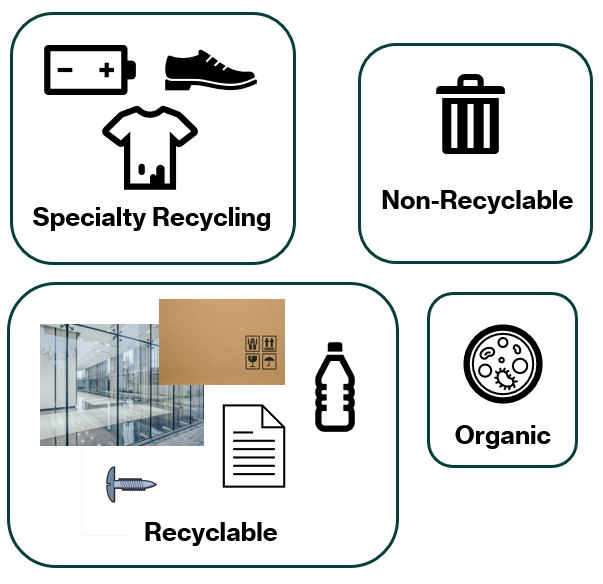
\includegraphics[width=0.8\linewidth]{dataset_classes.png}
    \caption{Item classification across garbage classes}
    \label{fig:dataset}
\end{figure}

\subsection{Model Architectures}
We evaluated three state-of-the-art Convolutional Neural Network (CNN) architectures, each representing a different, unique approach to balancing depth, efficiency, and representational power. These models were selected to explore architectures that have driven progress in image classification tasks:
\begin{itemize}
    \item \textbf{ResNet-50}: ResNet-50 is a deep residual network known for its robust feature extraction using skip connections. With 50 layers in depth, this architecture contains residual blocks that address the vanishing gradient problem and enable the model to learn complex features from images.
    \item \textbf{GoogLeNet (Inception v1)}: Notable for its computational efficiency through inception modules, this architecture won 1st place at the 2014 ImageNet Large Scale Visual Recognition Competition. In GoogLeNet, 1x1 convolution is used as a dimension reduction module to reduce computation, which can help increase depth and width. 
    \item \textbf{EfficientNet-B0}: This architecture is a compound-scaled model achieving a strong trade-off between performance and speed. Using compound scaling, this method is justified by the intuition that if the input image is bigger, then the network requires additional layers to increase the receptive field and requires more channels to caputer fine-grained details on the bigger image. 
\end{itemize}

Each model was trained using the same train-validation split and hyperparameter setup, ensuring a fair comparative evaluation.

% \begin{figure}[h]
%     \centering
%     % \includegraphics[width=0.8\linewidth]{images/model_architectures.png}
%     \caption{Architectural overview of ResNet, GoogLeNet, and EfficientNet used in the WISE pipeline.}
%     \label{fig:architectures}
% \end{figure}

\subsection{Training Configuration}
All models were trained on GPU-enabled hardware using the Adam optimizer and categorical cross-entropy loss. Early stopping and learning rate scheduling were applied to avoid overfitting and accelerate convergence.

\begin{table}[h]
\centering
\caption{Model Training Time}


\begin{tabular}{lc}
\hline
\textbf{Model} & \textbf{Training Time (s)} \\
\hline

GoogLeNet & 760 \\
ResNet-50 & 2136 \\
EfficientNet-B0 & 2471 \\

\hline
\end{tabular}
\label{tab:training_time}
\end{table}

\subsection{Evaluation Metrics and Insights}
\label{sec:evaluation}

To assess model performance, we evaluated each CNN architecture using two key metrics: classification accuracy and training time.

\begin{itemize}
    \item \textbf{GoogLeNet} was the \textit{fastest model} to train, completing in 760 seconds (12.67 minutes), but showed lower classification performance.
    \item \textbf{EfficientNet} delivered the \textit{best classification metrics}, although it had the longest training time at 2471 seconds (41.18 minutes).
    \item \textbf{ResNet} achieved a balance, performing well in both accuracy and efficiency, making it a robust and practical model for deployment.
\end{itemize}

\begin{table}[h]
\centering
\caption{Evaluation Metrics for CNN Models}
\
\renewcommand{\arraystretch}{1.2} %Adjust row height slightly
\begin{tabular}{|l|c|c|c|}

\hline
\textbf{\scriptsize Metric} & \textbf{\scriptsize GoogLeNet} & \textbf{\scriptsize ResNet50} & \textbf{\scriptsize EfficientNet} \\
\hline
Accuracy        & 0.966 & 0.955 & 0.871 \\
Precision       & 0.966 & 0.955 & 0.894 \\
Recall          & 0.966 & 0.955 & 0.871 \\
F1-Score        & 0.966 & 0.955 & 0.876 \\
Support         & 2944  & 2963  & 2963 \\
\hline
\end{tabular}
\label{tab:evaluation-smallheader}
\end{table}



These results help guide model selection based on use-case priorities—speed, accuracy, or a trade-off between the two. For real-world implementation, especially in environments with limited computational resources or real-time constraints, such insights are critical.




%%%%%%%%%% EXPERIMENTS %%%%%%%%%%%%%%
\section{Experiments and Results}
\label{sec:experiments}
Training times varied significantly: ResNet took 2136 seconds, GoogLeNet 760 seconds, and EfficientNet 2471 seconds. ResNet achieved the best classification metrics, while GoogLeNet trained fastest, but underperformed in accuracy. EfficientNet performed worst across the board. These results indicate a trade-off between speed and accuracy in real-world deployment scenarios.

%%%%%%%%%% DISCUSSION %%%%%%%%%%%%%%
\section{Discussion}
\label{sec:discussion}
ResNet emerged as the most balanced choice for deployment due to its superior classification metrics, despite its longer training time. The performance of the models varied by class complexity, highlighting the need for robust architectures in applications such as smart bins or automated recycling plants. 

GoogLeNet’s speed advantage may suit edge devices, where real-time analysis of object type detection and classification into garbage types are time sensitive.

EfficientNet requires more tuning for improvement. It is possible that each of these models do well in specific parts of the feature space of the images we have. So having an educated ensemble of the models would be beneficial to have an overall winner prediction framework. 

%%%%%%%%%% CONCLUSION %%%%%%%%%%%%%%
\section{Conclusion and Future Work}
\label{sec:conclusion}
The WISE project validated the potential of CNNs for waste classification. ResNet’s performance makes it suitable for real-world deployment, including smart waste bins and mobile applications. 

Future work could explore transfer learning, data augmentation, and real-time deployment using embedded systems.

For an industrial product out of this project, we will need to experiment the ensemble model on high volume of images across various lighting settings to ensure all edge cases are covered. Having confidence intervals of predictive capabilities will help the users can make an informed decision in case of ambiguous situations.



%\bibliographystyle{plainnat}
\begin{thebibliography}{99}
\bibitem{chen2023}
Chen, A., Liu, Y., \& Zhang, Q. (2023).
\textit{Image-Based Waste Classification Using Lightweight CNNs.}
International Journal of Environmental AI, 15(2), 122-135.
\bibitem{choi2023}
Choi, J., Lim, B., \& Yoo, Y. (2023). 
\textit{Advancing plastic waste classification and recycling efficiency: Integrating image sensors and deep learning algorithms.}
Applied Sciences, 13(18), 10224.
\end{thebibliography}

\appendix
\section{Appendix (Optional)}
Details about hyperparameters, training configurations, and confusion matrices can be included here if needed.

\end{document}
